%% The Appendices part is started with the command \appendix;
%% appendix sections are then done as normal sections
\newpage
\appendix
\section{Values of material properties used in the simulations}\label{sec:Tables}
% The linear elastic properties of Homalite-100:
% Table~ for elastic properties of Homalite-100
\begin{table}[H]
    \centering
    \begin{tabular*}{0.8\textwidth}{ @{\extracolsep{\fill}} cccccc}
    \toprule
    $G\ [\mathrm{GPa}]$ & $\nu$ & $\alpha$ &  $M\ [\mathrm{GPa}]$ & $\kappa\ [\mathrm{m^2/(Pa\cdot s)}]$ & $c [\mathrm{m^2/s}]$\\
    \midrule
    $10$ & $0.24$ & $0.5530$ & $0.35$ & $2.1688\times10^{-19}$ & $1.0\times10^{-8}$ \\
    \bottomrule
    \end{tabular*}
    \caption{Linear poroelastic material properties of the bulk material}
    \label{tab:elasticBulk}
\end{table}

% Rate-and-state friction properties of Homalite-100 interfaces:
% Table~ for rate-and-state properties
\begin{table}[H]
    \centering
    \begin{tabular*}{0.9\textwidth}{ @{\extracolsep{\fill}} ccccccc}
    \toprule
    $f_*$ & $V_*\ [\mathrm{m/s}]$ & $a$ & $b$ & $D_{RS}\ [\mathrm{m}]$ & $\kappa_{cx}\ [\mathrm{m^2/(Pa\cdot s)}]$ & $\kappa_{cy}\ [\mathrm{m^2/(Pa\cdot s)}]$\\
    \midrule
    $0.55$ & $1.0\times 10^{-6}$ & $0.0112$ & $0.0160$ & $16.75\times 10^{-6}$ & 8.75834 \times 10^{-11} & 8.75834 \times 10^{-20}\\
    \bottomrule
    \end{tabular*}
    \caption{Friction and diffusivity properties of the fault interface}
    \label{tab:fricPropsFault}
\end{table}

\section{Supplementary figures}
\begin{figure}[htbp]
    \centering
    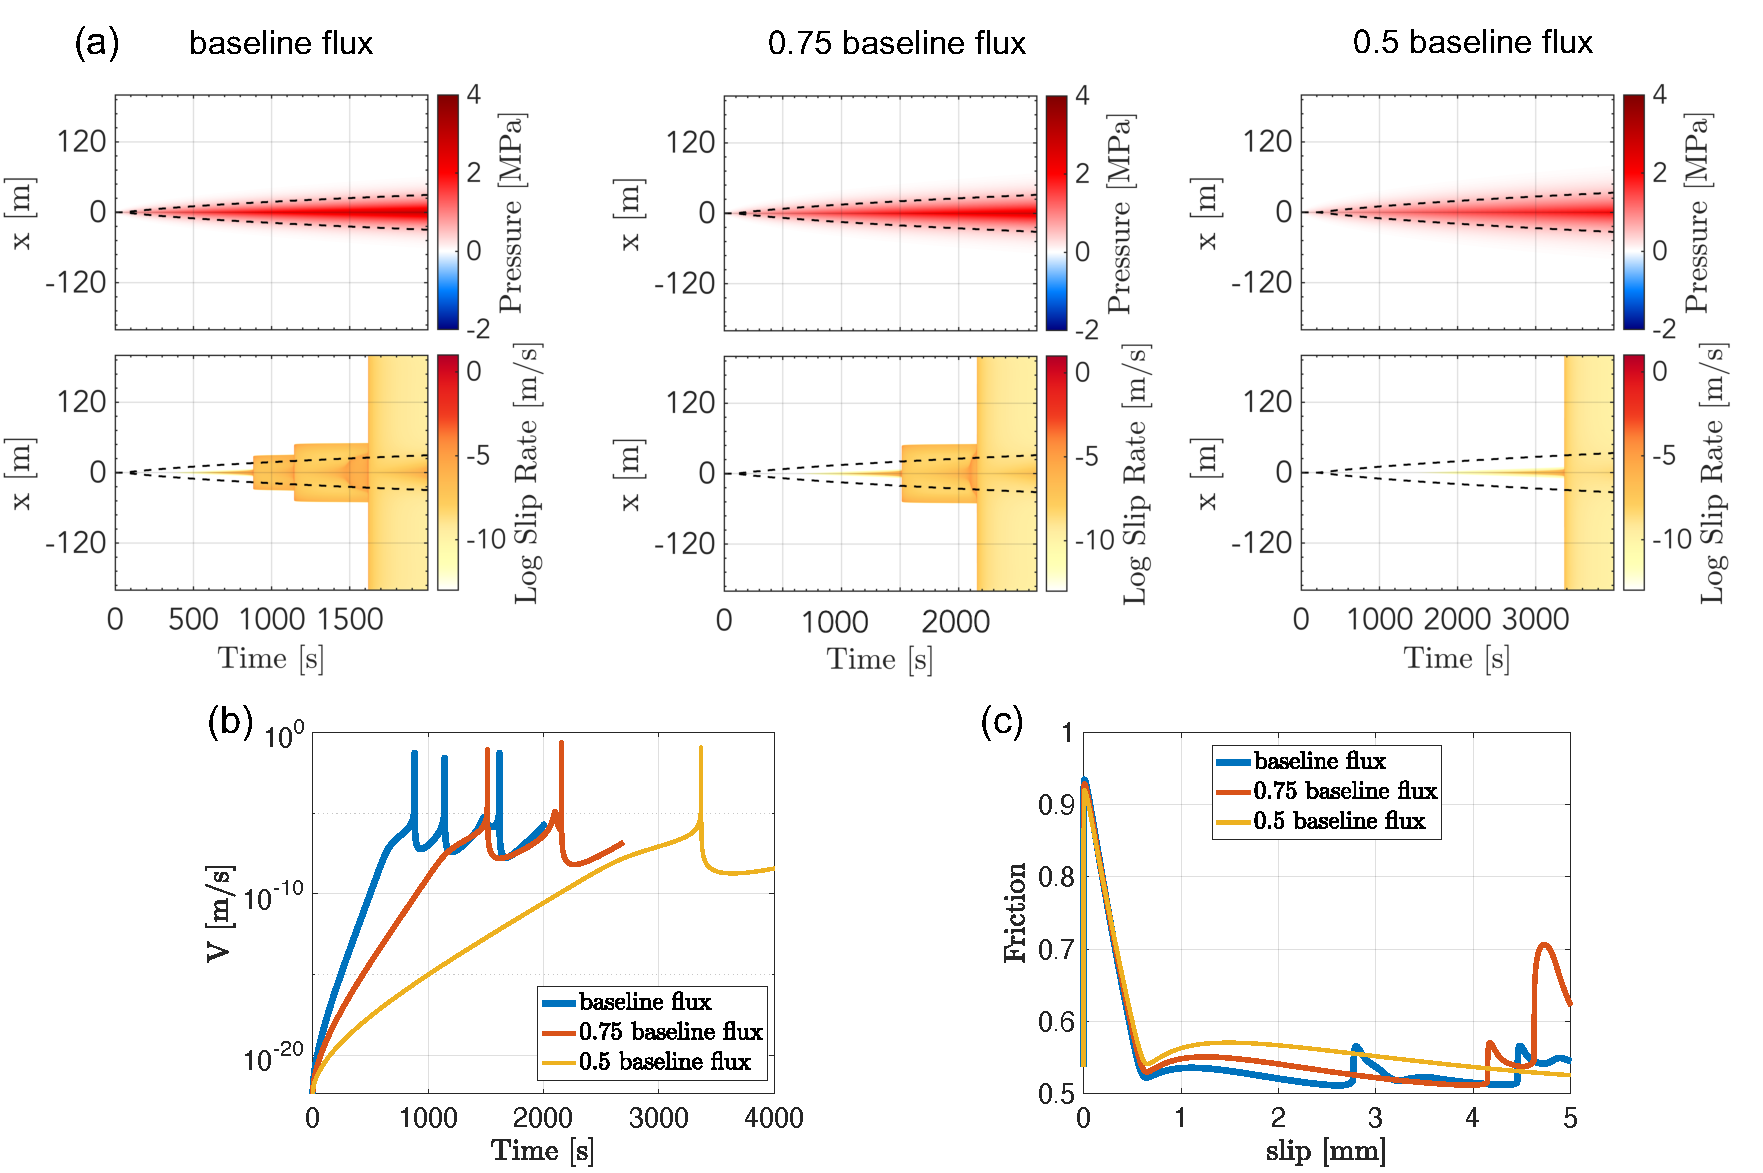
\includegraphics[width=1.0\textwidth]{figures/flux_elast_0.24.pdf}
    \caption{The effect of injection rate (flux) on stability of fault slip surrounded by elastic, permeable bulk with $\nu = 0.24$. 
    The total injected mass is kept the same for all cases, 
    and thus time is adjusted for different injection rate. 
    Baseline flux is set to be $1.0\times10^{-4}\ \mathrm{Kg / (m \cdot s)}$.
    (a) Pore fluid pressure change and slip vs. time along $x$ for baseline flux, $0.75$ baseline flux and $0.5$ baseline flux. 
    (b) Slip rate vs. time at $x = 0\ \mathrm{m}$ for the above 3 cases. 
    (c) Friction vs. slip at $x = 0\ \mathrm{m}$ for the above 3 cases.}
    \label{fig:fluxElas0.24}
\end{figure}

\begin{figure}[htbp]
    \centering
    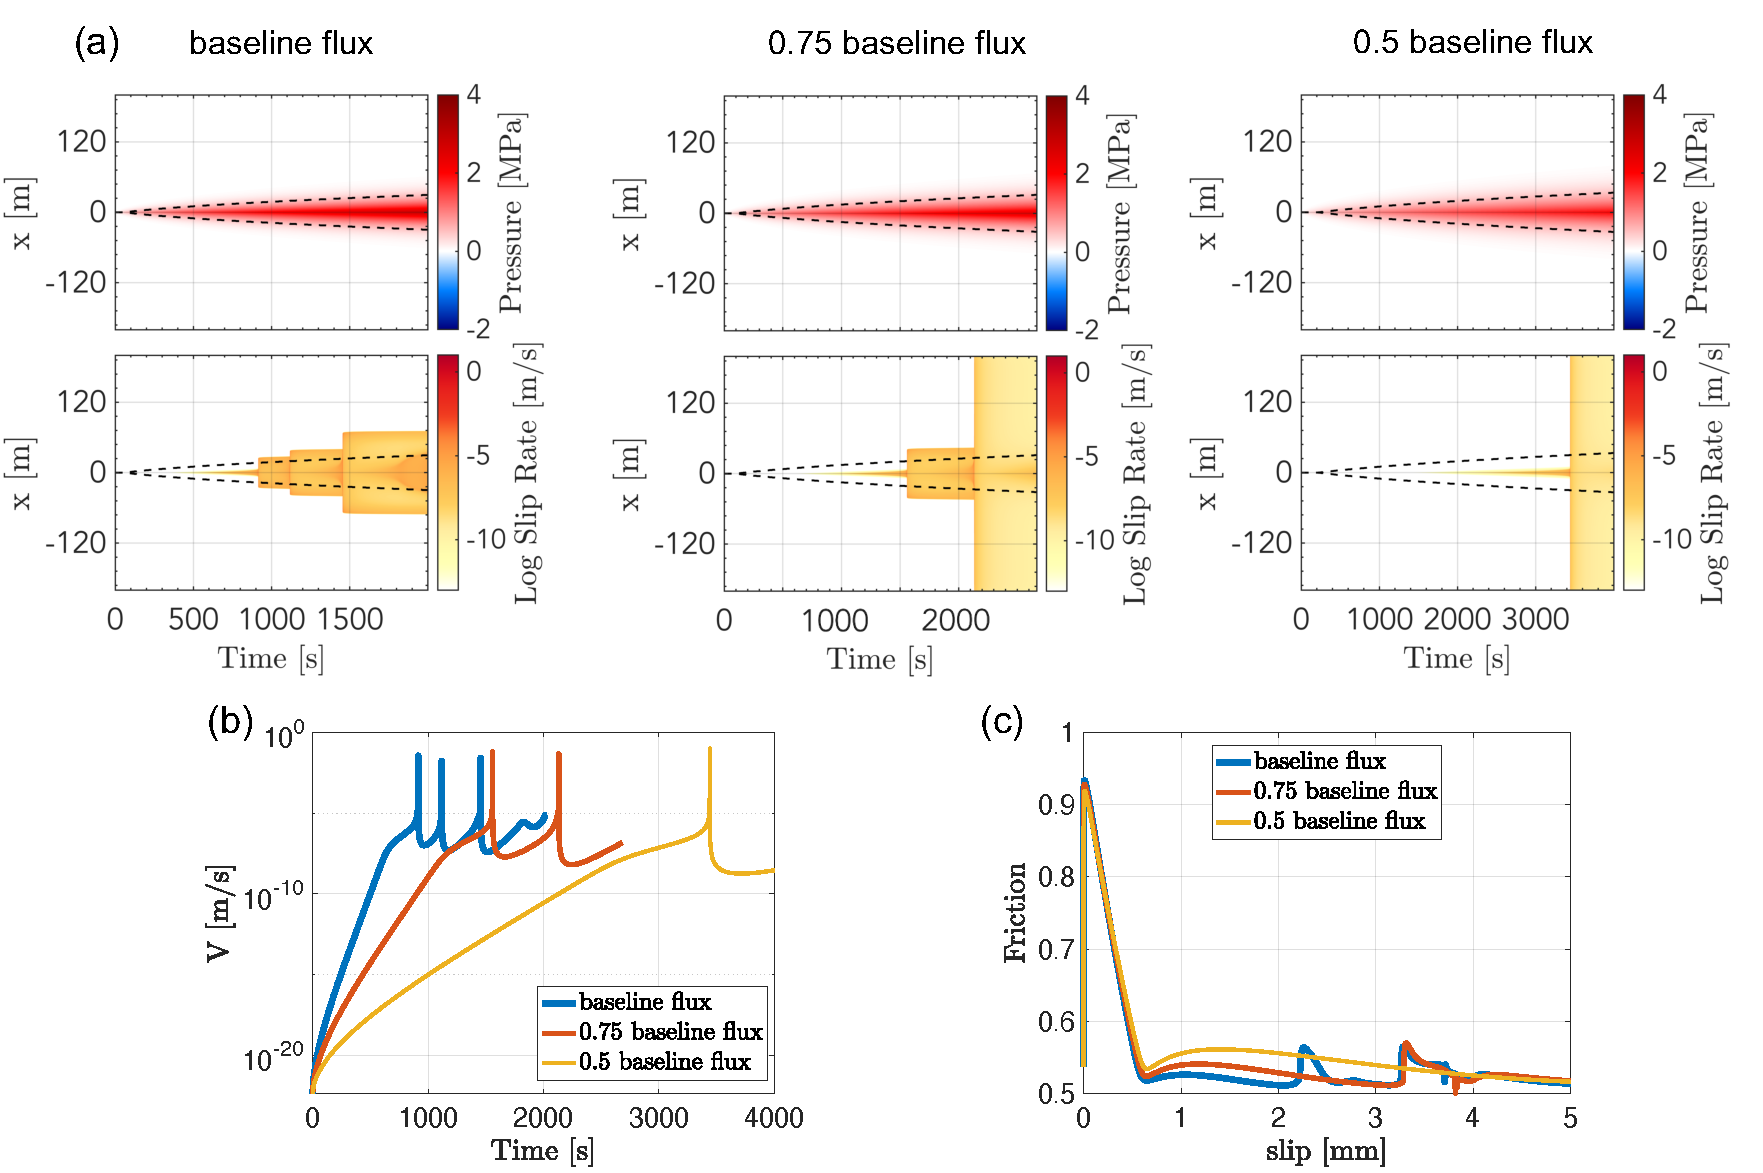
\includegraphics[width=1.0\textwidth]{figures/flux_elast_0.35.pdf}
    \caption{The effect of injection rate (flux) on stability of fault slip surrounded by elastic, permeable bulk with $\nu = 0.35$. 
    The total injected mass is kept the same for all cases, 
    and thus time is adjusted for different injection rate. 
    Baseline flux is set to be $1.0\times10^{-4}\ \mathrm{Kg / (m \cdot s)}$.
    (a) Pore fluid pressure change and slip vs. time along $x$ for baseline flux, $0.75$ baseline flux and $0.5$ baseline flux. 
    (b) Slip rate vs. time at $x = 0\ \mathrm{m}$ for the above 3 cases. 
    (c) Friction vs. slip at $x = 0\ \mathrm{m}$ for the above 3 cases.}
    \label{fig:fluxElas0.35}
\end{figure}